%%%%%%%%%%%%% ptdr definitions %%%%%%%%%%%%%%%%%%%%%
\input{ptdr-definitions}

\newcommand{\pp}{\ensuremath{\mathrm{pp}}}%
\newcommand{\Wo}{\ensuremath{\mathrm{W}}}%
\newcommand{\Zo}{\ensuremath{\mathrm{Z}}}%
\newcommand{\rts}{\ensuremath{\sqrt{s}}}%
\newcommand{\ra}{\ensuremath{\rightarrow}}%
\newcommand{\MN}{\ensuremath{\mu\nu}}%
\newcommand{\MW}{\ensuremath{\mathrm{m}_\Wo}}%
\newcommand{\MZ}{\ensuremath{\mathrm{m}_\Zo}}%
\newcommand{\MT}{\ensuremath{\mathrm{M}_T}}%

\newcommand{\Wmn}{\ensuremath{\Wo \ra \MN}}%
\newcommand{\Zmm}{\ensuremath{\Zo \ra \MM}}%
\newcommand{\Wtn}{\ensuremath{\Wo \ra \tau\nu}}%
\newcommand{\Ztt}{\ensuremath{\Zo \ra \tau\tau}}%
\newcommand{\ppZmm}{\pp \ra \Zo + X \ra \MM + X}%
\newcommand{\ppWmn}{\pp \ra \Wo + X \ra \MN + X}%



%%%%%%%%%%%%%%%  Title page %%%%%%%%%%%%%%%%%%%%%%%%


\cmsNoteHeader{XXX/YYY}


\title{Study of the Barrel RPC L1 Trigger efficiency \\
with a muon sample triggered by the DT system}
% Force line breaks with \\

%Author is always "The CMS Collaboration" for PAS, so author, etc will be ignored
\address[nap]{INFN and Universita' di Napoli}
\address[bari]{INFN and Universita' di Bari}
\author[nap]{F.~Fabozzi}
\author[nap]{A.O.M.~Iorio}
\author[nap]{P.~Paolucci}
\author[bari]{R.~Trendadue}

% please supply the date in yyyy/mm/dd format. Today has been
% redefined to do so, but it should be fixed as of the final release date.
%\date{\today}

% note that you cannot use \verb in the abstract text
\abstract{
    We present a study of the L1 trigger efficiency for RPCs in the
    Barrel of the CMS Muon System. The method exploits the independency of the
    DT and RPC trigger systems. Muon tracks in the event are 
    triggered and reconstructed using the DT system only, and for each of
    them we search for a compatible RPC L1 trigger object. 
    We discuss in detail the results obtained on a few good 
    runs taken from CRAFT08 and CRAFT09 datasets. The algorithm has been 
    released in the Prompt Analysis Framework of the RPC system for a fast
    off-line monitoring of the trigger performances.
}

% these need to be filled in by hand and should (MUST) match the info
% in the TeX equivalents less the TeX markup
%\hypersetup{%
%pdfauthor={Francesco Fabozzi},%
%pdftitle={Towards a measurement of W and Z cross sections into muons in pp collisions at rts=10 TeV},%
%pdfsubject={CMS},%
%pdfkeywords={CMS, physics, software, computing}}

\maketitle %maketitle comes after all the front information has been supplied

%%%%%%%%%%%%%%%%%%%%%%%%%%%%%%%%  Begin text %%%%%%%%%%%%%%%%%%%%%%%%%%%%%
\section{Introduction}
The CMS Muon System~\cite{ref:mutdr}\cite{ref:jinst} has 
been designed to provide excellent muon
identification, triggering and precise momentum reconstruction 
over the entire kinematic range foreseen at LHC. A crucial
feature of the system is the redundancy provided by the DT/RPC 
(CSC/RPC) independent sub-systems in the Barrel (Endcap) region.
In particular, the RPC system is able to provide 
a fast and higly segmented trigger, with a 
sharp \pt threshold, in the rapidity range $|\eta| < 1.6$.
The independence of the DT and RPC systems can be exploited
to develop a method for the measurement of the Barrel RPC L1 
trigger efficiency, which can be extremely useful 
for a prompt monitoring of system performances.
In this note we discuss this method and present results
obtained on CRAFT08 and CRAFT09 cosmic data samples.

\section{The Barrel RPC system}
In this section we briefly describe the layout of the
Barrel RPC system just to introduce some
naming conventions. Detailed descriptions
can be found in References \cite{ref:mutdr}
and \cite{ref:jinst}.

The Barrel Muon System is composed of 5 Wheels along 
the $z$ direction, named W-2, W-1, W0 (the central one), 
W+1, W+2. Each wheel is divided into twelve 
sectors (with approximately dodecagonal geometry in the 
$r$-$\phi$ view), from sector S01 to sector S12 
(see Fig.~\ref{fig:barrel_lay}).

\begin{figure}[hbtp]
  \begin{center}
    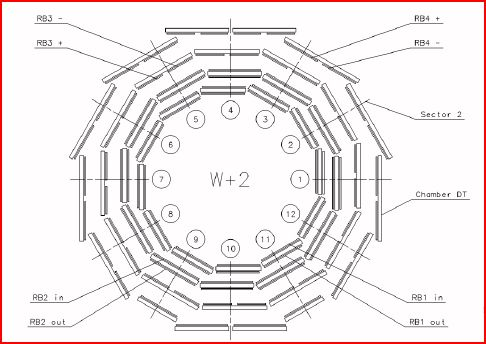
\includegraphics[width=0.8\textwidth]{barrel_layout}
    \hspace{1cm}
    \caption{Transverse view of the Barrel RPC system.}
    \label{fig:barrel_lay}
  \end{center}
\end{figure}

For each sector there are 4 DT stations, inserted in the 
iron gaps of the Barrel Yoke, from MB1 (the inner one)
to MB4 (the outer one). 

The RPC stations are mounted on one or both sides of the DT 
stations. Station MB1 is provided with RPC stations on 
bottom and top sides (RB1In and RB1Out stations), same 
for MB2 (RB2In and RB2Out stations). Stations MB3 and MB4
are provided with RPC stations on the bottom side only
(RB3 and RB4 stations). 
With this design, a total of six concentric RPC layers are 
available in the Barrel Muon System. The inner
layers can provide up to four coordinate measurements also for 
low momentum tracks crossing only MB1 and MB2 stations.

For each RPC station, pick-up strips running parallel to the 
beam axis provide coordinate measurement in the $r$-$\phi$ view,
thus allowing \pt measurement of the track. 
Segmentation in the $\eta$ view is obtained by sectioning
a plane of strips in two or three parts. 
The $\eta$ partitions are called {\em rolls}.
An RPC station can be segmented into two rolls (named Backward and 
Forward) or three rolls (named Backward, Middle, and Forward).
RPC stations 3 and 4 present also a segmentation along $\phi$ in two 
partitions ( named + and - ). RPC Station 4 sector 4 is segmented in 4 $\phi$ partitions.

\section{The L1 trigger system for Barrel RPCs}
From the point of view of the L1 trigger~\cite{ref:trig_tdr}, 
the RPC system volume is logically partitioned into 
sections. L1 trigger objects are searched 
for independently in each section.
Sections in the $\eta$ view will be referred as {\em towers},
and for each tower the partitions in  
the $r$-$\phi$ view will be referred as {\em cones}.


\subsection{Trigger towers}
\label{sec:trig_towers}
The definition of the $\eta$ boundaries 
of towers (see Fig.~\ref{fig:eta_towers}) is based on a set 
of reference layers.

\begin{figure}[hbtp]
  \begin{center}
    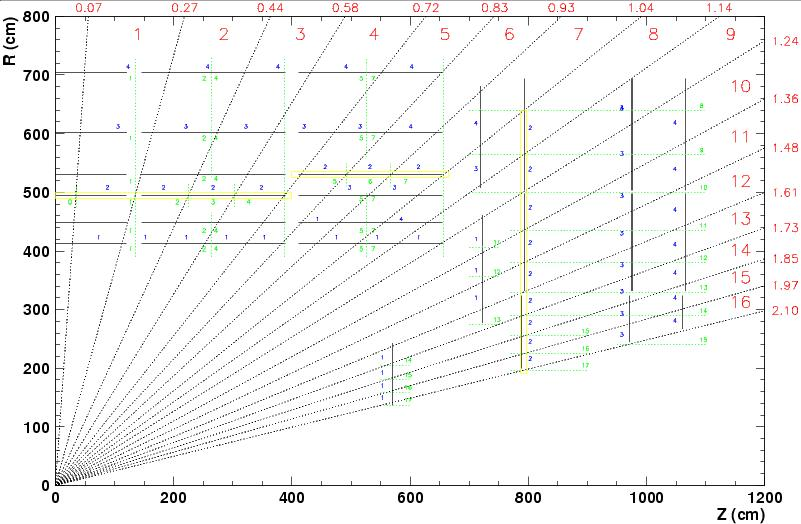
\includegraphics[width=0.8\textwidth]{eta_towers}
    \hspace{1cm}
    \caption{Trigger eta towers.}
    \label{fig:eta_towers}
  \end{center}
\end{figure}

In the Barrel, the reference layers are:
layer RB2In for W+1, W0, and W-1, 
and layer RB2Out for W-2 and W+2. 
Each tower must contain only one entire roll 
of a reference layer. On the 
other hand, a roll of a non-reference layer
can belong to adjacent towers, thus in this case 
the association of roll to towers is not univocally defined. 
The RPC trigger logic has a total of 17 towers.
A total of 5+5+1 towers are entirely contained in the Barrel.

\subsection{Trigger cones}
On the reference layers, the strips are grouped in
non-overlapping sets of 8 adjacent strips called {\em segments}.
Each segment subtends a $\phi$ angle of $2.5^\circ$, for a total 
of 144 segments (12 segments for each sector).
Each cone must contain only one segment of a reference 
layer.
On the other hand, in non-reference layers a larger number
of strips is grouped into a segment, so that a segment
covers more than $2.5^\circ$ in those layers.
Thus adjacent segments overlap in the non-reference layers and 
the association of a strip to those segments is not univocally defined.

\subsection{The L1 PACT logic}
The PAttern COmparator Trigger (PACT) logic 
collects RPC hits from all stations and searches for
spatial and time coincidences independently
in each cone. The $\eta$ and $\phi$ coordinate of the trigger
objects are assigned on the reference station.
By comparison with predefinite patterns of hits, 
also a \pt value is assigned to the candidate trigger 
object. 

Due to the overlap of adjacent cones, 
{\em ghost} trigger objects in a certain $\eta$ tower 
can appear. Ghosts can also appear in adjacent towers 
due to the sharing of the rolls in non-reference stations. 
For this reason, trigger candidates are processed by a proper 
ghost identification and removal logic,
and the remaining ones are sorted according to quality criteria.
More details can be found in Ref.~\cite{ref:trig_tdr}.

Finally, the 4 highest \pt muons
from the Barrel and the 4 highest \pt muons from the
Endcap are sent to the Global Muon Trigger.

\subsection{Cosmic patterns in PACT}
In order to increase the trigger efficiency for 
cosmic muons, which are not constrained
to come from the interaction vertex, 
a looser pattern definition has been 
adopted with respect to collision runs.
A cosmic pattern is defined as a 
time coincidence of hits on at least
3 different RPC stations in a cone (3/6 majority).
No different patterns as a function 
of \pt are defined, thus the system is
not able to assign a \pt value 
to the track.

\section{Analysis method}
We start from a sample of reconstructed tracks 
in the Muon System which are matched to a DT 
trigger object. In this way we reject fakes 
and define a sample of muons tracks that have not been 
triggered exclusively by RPCs.

If the number of tracks in the sample is 
$N_{match}^{DT}$, and under the assumption
that RPC and DT triggers are uncorrelated,
the RPC trigger efficiency 
$\epsilon_{L1}^{RPC}$ is given by the fraction 
of tracks in the sample that are matched also 
to an RPC trigger object:
\begin{equation}
\epsilon_{L1}^{RPC} = N_{match}^{RPC\&DT}/N_{match}^{DT} \,\,\,.
\end{equation}

\subsection{Tracks selection}
For the analysis we use a collection of CosmicMuons.
CosmicMuons are made of tracks reconstructed in the
Muon System only .
The two legs of a muon which traverses
the Tracker System are reconstructed as two separate 
CosmicMuon tracks.
In order to prevent an eventual bias due to tracks 
that would not have been reconstructed without
RPC hits, we re-run the reconstruction using DT only.

We select cosmic tracks pointing to the $p$-$p$ interaction
region by requiring that the track passes through a cylinder 
centered in the interaction point, with the height parallel 
to the z axis $h = 260 cm$ and a radius $r = 90 cm$ 
(definition of TrackerPointing skim). In addition, we apply the following 
cuts:
\begin{itemize}
\item
$\pt$ at the innermost point $ > 5$\GeVc 
\item
$N_{hits}$ in the DT $ > 20 $;
\item
$\chi^2$ of the track fit $ < 20 $.
\end{itemize}
The \pt cut removes tracks which are
looping in the transverse plane due 
to the magnetic field. The last two cuts 
ensure good quality of the DT reconstruction 
and prevent an eventual bias due to 
tracks that would not have been triggered 
without RPC hits.
Figures ~\ref{fig:pttrack} and ~\ref{fig:nhitschi2} show 
the distributions of these variables for typical pointing
CosmicMuon tracks.

\begin{figure}[hbtp]

     \begin{minipage}{1.0\textwidth}
     \begin{center}
      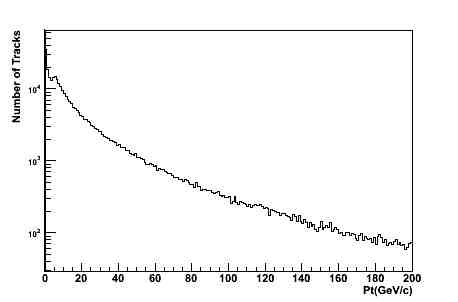
\includegraphics[width=0.8\textwidth]{pt_sta}
       \caption{ 
Distribution of the \pt of the cosmic muon tracks. 
}
      \label{fig:pttrack}
  \end{center}
  \end{minipage}
     
 \begin{minipage}{1.0\textwidth}
  \begin{center}
 
     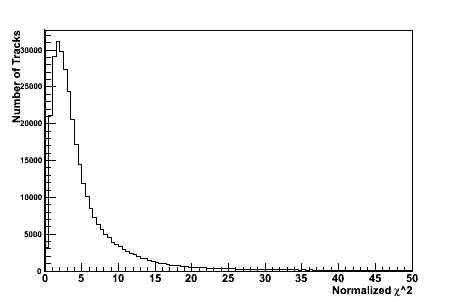
\includegraphics[width=0.4\textwidth]{chi2_sta}
     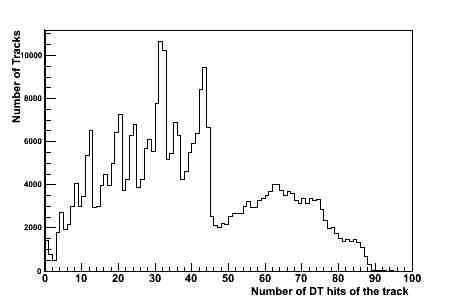
\includegraphics[width=0.4\textwidth]{num_hits_sta}
\caption{Distribution of the normalized $\chi^2$ (left) and number of DT hits (right) 
of the cosmic muon tracks. The tracks with $< 5$ hits
are reconstructed through the CSCs chambers. 
All distributions are taken before the cuts were applied.
}
      \label{fig:nhitschi2}
  \end{center}
  \end{minipage}

\end{figure}

\subsection{Track matching with trigger objects}
The position in $\eta - \phi$ of the L1 trigger for both DTs and RPCs is defined
on the reference layer. The RPC reference layers have been described
in Sec.~\ref{sec:trig_towers}. The DT reference layer is Station 2 
of each wheel. Thus, in order to match the track to a DT trigger candidate, 
the track is extrapolated to MB2.
The extrapolation is done by taking the last point of the track and 
propagating backwards to the reference layer using 
the {\em SteppingHelixPropagator},
an accurate propagation method through the CMS detector
geometry which takes into account the magnetic field, 
the energy loss in the detector material and the 
multiple scattering~\cite{ref:muonreco_note}.
%The distributions of $\eta$ and $\phi$ at the reference 
%station for the tracks are shown in Fig. ~\ref{fig:track_eta_phi} 

The track-trigger matching is performed in the $\phi$ coordinate 
only, which is the most accurate coordinate measured by both 
DT and RPC trigger systems. It was not possible to use a matching
in $\eta$ with the L1 DT trigger candidates since the $\eta$ part
of the algorythm was not commissioned yet during CRAFT08 data taking. 
The $\phi$ distributions for DT and RPC trigger
objects are shown in Fig.~\ref{fig:trigger_eta_phi}

\begin{figure}[hbtp]
  \begin{center}
    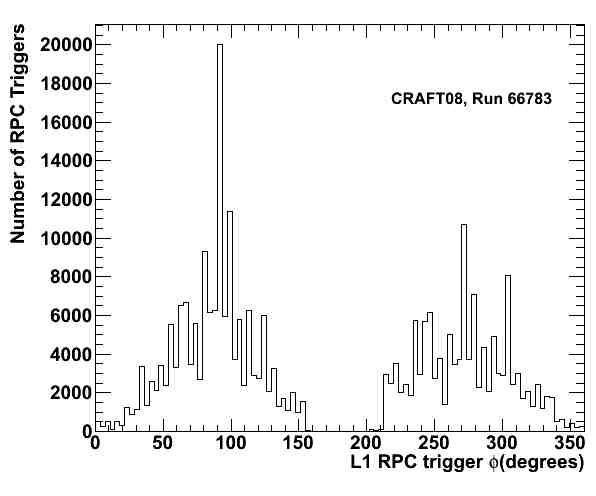
\includegraphics[width=0.4\textwidth]{phi_rpc}
    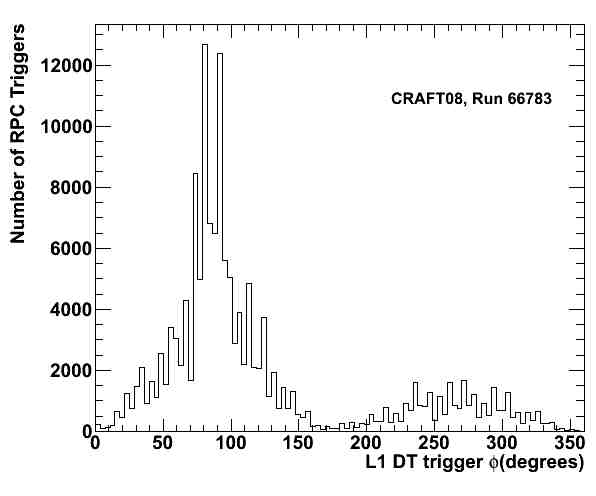
\includegraphics[width=0.4\textwidth]{phi_dt}
      \caption{Phi distribution of the RPC (left) and DT (right) triggers.}
    \label{fig:trigger_eta_phi}
  \end{center}
\end{figure}

The matching requirement is $|\Delta\phi_{t-DT}| < 30^\circ$,
where $\Delta\phi_{t-DT}$ is the difference 
between the $\phi$ of the track at the reference layer and
the $\phi$ of the DT trigger. This loose requirement
provides a high matching efficiency.

If we find a match with a DT trigger, then we proceed
for matching to an RPC trigger. 
Figure~\ref{fig:trigger_residuals} shows the overall $\Delta\phi_{t-RPC}$ as measured 
using both cosmic patterns and collision patterns (the
last one obtained by running the trigger emulator).
The second peak at $\Delta\phi_{t-RPC} \approx -0.06$ for the residuals distribution 
of cosmics patterns is due to the fact that the cosmics 
pattern configuration cannot identify the \pt of the track.
In case of two candidates with the same quality then the one
with the smaller $\phi$ is selected.

\begin{figure}[hbtp]
  \begin{center}
    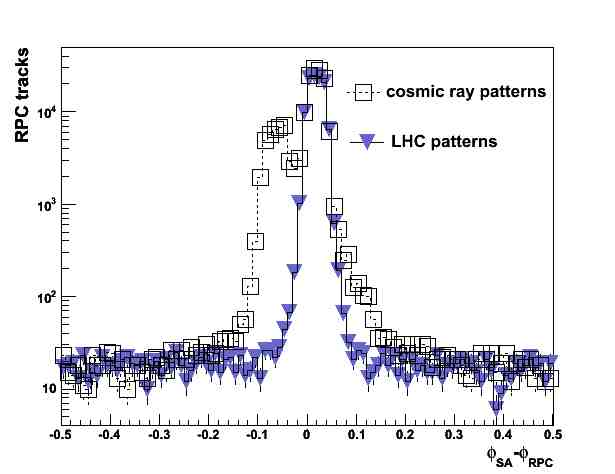
\includegraphics[width=0.8\textwidth]{residuals_rpc}
    \hspace{1cm}
    \caption{Distribution of the difference between the $\phi$ of the track measured 
    at the reference station and the $\phi$ of the RPC trigger (Run 66783).}
    \label{fig:trigger_residuals}
  \end{center}
\end{figure}

The matching requirement is $|\Delta\phi_{t-RPC}| < 30^\circ$,
where $\Delta\phi_{t-RPC}$ is the difference 
between the $\phi$ of the track at the reference layer 
and the $\phi$ of the RPC trigger.

\section{Data samples}
Only cosmic tracks which mimic muons from collisions
have been considered for this study. 
For this reason, we have analized runs taken from the 
following CRAFT08 and CRAFT09 datasets:
\begin{itemize}
\item
Commissioning08\/2213\_Tosca090322\_2pi\_scaled\_ReReco\_FromTrackerPointing-v1\/RAW-RECO
\item
Cosmics\/CRAFT09-PromptReco-v1\/RECO
\end{itemize}

The CRAFT08 dataset is a TrackerPointing skim, that is 
only cosmics pointing to the primary vertex 
region of CMS are selected. 
On the contrary, the CRAFT09 dataset is non-skimmed, 
since the pointing skim was not yet 
available. In this case we have filtered the 
events at the analysis level by applying the same
requirements used in the pointing skim.
Table~\ref{tab:runs} reports the run numbers analyzed and the 
relevant detector conditions.
%In these runs all the RPCs towers are included in the trigger. 

 \begin{table}[htb]
    \begin{center}
      \begin{tabular}{|c|c|c|c|c|} \hline
Dataset & Run   & RPC HV & Average Barrel RPC eff.\\ \hline
CRAFT08 & 66783 & 9.2 kV & $82.41\%$ \\ \hline
CRAFT09 & 110409  & 9.4 kV & $92.05\%$ \\ \hline
CRAFT09 & 110419  & 9.4 kV & $91.67\%$ \\ \hline
      \end{tabular}
      \caption{Analyzed runs from CRAFT08 
and CRAFT09 datasets. HV value and average
efficiency for the barrel RPCs are also reported.}
    \label{tab:runs}
    \end{center}
  \end{table}

\section{RPC trigger efficiency}
\label{resultSection}

%For CRAFT08 and CRAFT09 respectively we consider two datasets in which all 

%the RPCs towers are included in the trigger. 
We study the trigger efficiency with respect to the \pt of the track and 
with respect to the position of the track on the reference layer.

\subsection{Results for CRAFT08}
\label{eff_08}
Figures~\ref{fig:eff_eta_phi_top_08},~\ref{fig:eff_eta_phi_bot_08} show 
the RPC trigger efficiency in the Barrel as a function of the 
$\eta - \phi$ of the track on the reference layer, for the top 
and bottom part of the detector respectively. 
Note that sectors 1 and 7 are splitted in half through the 
two plots, since sector 1 covers the $\phi$
region from $-15^\circ$ to $15^\circ$.

\begin{figure}[hbtp]
  \begin{center}
     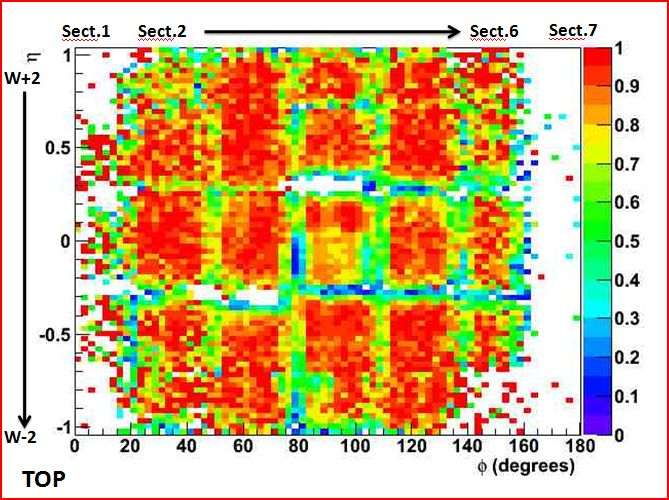
\includegraphics[width=0.9\textwidth]{eff_eta_phi_top_08_new}
      \hspace{1cm}
      \caption{RPC trigger efficiency in CRAFT08 as a function of $\eta$ and $\phi$ 
      for tracks in top part of the Barrel detector 
      ($ 0^\circ < \phi < 180^\circ $). The $\eta$ and $\phi$
      coordinates are extrapolated to the reference layer.
      The wheels (sectors) corresponding to different $\eta$-$\phi$
      regions are labelled on the left (top) part of the plot.
      }
    \label{fig:eff_eta_phi_top_08}
  \end{center}
\end{figure}

\begin{figure}[hbtp]
     \begin{center}
      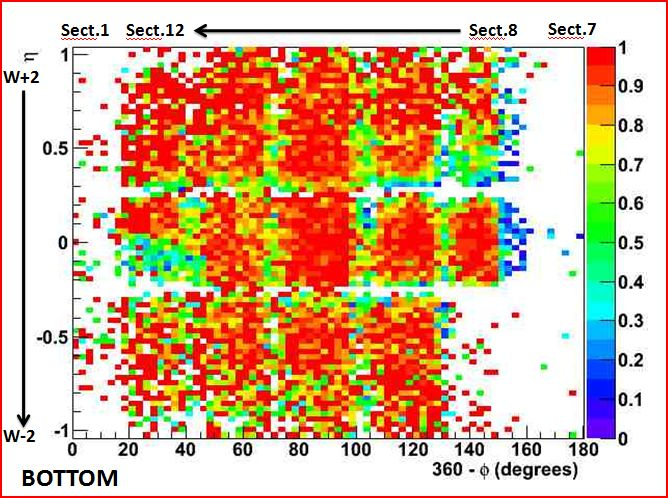
\includegraphics[width=0.9\textwidth]{eff_eta_phi_bot_08_new}
      \hspace{1cm}
      \caption{RPC trigger efficiency in CRAFT08 as a function of $\eta$ and $\phi$ 
      for tracks in bottom part of the Barrel detector 
      ($ 180^\circ < \phi < 360^\circ $). The $\eta$ and $\phi$ coordinates are 
      extrapolated to the reference layer. 
      Note that the variable plotted on the x-axis is 
      $360^\circ - \phi$. The wheels (sectors) corresponding to different $\eta$-$\phi$
      regions are labelled on the left (top) part of the plot.
      }
    \label{fig:eff_eta_phi_bot_08}
  \end{center}
\end{figure}

The efficiency of the trigger drops in the regions
of separation between two adjacent sectors or wheels,
and in particular it is evident the effect of having
shorter chambers in W+1\_Sect.4 and W-1\_Sect.3 due to 
chimneys.

There are some regions that appear to be less populated.
This is due to several reasons: cosmic particles 
distribution which disfavours vertical sectors
(sectors 1 and 7), hardware/trigger problems in CRAFT08
such as DT triggers OFF (W-2\_Sect.6),
masked RPC channels (sectors 6, 7, 8, W-2\_Sect.9,
W-1\_Sect.9). Note also that the loose trigger 
matching condition of $30^\circ$
gives some statistics in these regions
when the RPC/DT trigger object is found in an adjacent
sector.

It is also worthwhile to note that in W0\_Sect.4 the RB3 layer
had low detection efficiency in CRAFT08 (due to a readout problem), 
and this reflects in a lower trigger efficiency than other sectors.

In order to determine the trigger efficiency vs. \pt, we 
introduce geometrical cuts in order to select only cosmic 
tracks in the central regions of the rolls and sectors.
Indeed, in the border regions DT and RPC triggers are
affected by common inefficiencies due to geometry, which
introduces correlations between the two systems.
The choice of the fiducial cuts is shown in Table~\ref{tab:volumecuts}. 

 \begin{table}[htb]
    \begin{center}
      \begin{tabular}{|c|c|} \hline
  $   |\phi - \phi_{center} | < 5^o $ & \\ \hline
  $  |z| < 100 or 200 < |z| < 300 or 450 < |z| < 550$  &  \\ \hline
      \end{tabular}
      \caption{Volume cuts applied to select tracks in the center of the 
      rolls and sectors. $\phi_{center}$ is the value of $\phi$ at the 
      center of the sector. 
      }
    \label{tab:volumecuts}
    \end{center}
  \end{table}

The trigger efficiency vs. the $\pt$ of the tracks is shown 
in Fig.~\ref{fig:eff_pt_08}.
The efficiency reachs a plateau at around $40 \GeVc$ 
at a value of $\epsilon_{08} = 88.98 \pm 0.33 % $.

\begin{figure}[hbtp]
  \begin{center}
    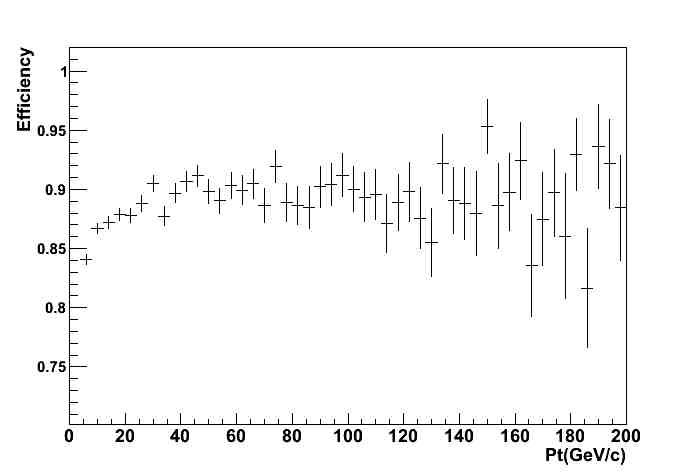
\includegraphics[width=0.8\textwidth]{eff_pt_08}
    \hspace{1cm}
    \caption{Trigger efficiency vs \pt of the tracks.}
    \label{fig:eff_pt_08}
  \end{center}
\end{figure}

\subsubsection{Comparison with Tag and Probe method}
We have compared the CRAFT08 trigger efficiency
measured with the DT vs. RPC method with the efficiency measurement 
based on the Tag and Probe method~\cite{ref:mupaper}. 
The comparison was made between the efficiencies measured 
in the top part of the detector, since in the Tag and Probe
technique tracks in the bottom part were used for the tagging.
The comparison is shown in Table~\ref{tab:notecomparison}.
The level of agreement is quite good.

 \begin{table}[htb]
    \begin{center}
      \begin{tabular}{|c|c|} \hline
Tag \& Probe & $88.02 \pm 0.22 $ \\ \hline
DT vs RPC & $87.93 \pm 0.38 $  \\ \hline
     \end{tabular} 
      \caption{Overall RPC trigger efficiency in the top part of the Barrel
evaluated with the Tag $\and$ Probe and DT vs. RPC methods.}
    \label{tab:notecomparison}
    \end{center}
  \end{table}

\subsection{Results for CRAFT09}
\label{eff_09}
Figures~\ref{fig:eff_eta_phi_top_09} and \ref{fig:eff_eta_phi_bot_09}
show the trigger efficiency in bins of $\eta - \phi$ of the 
track, extrapolated to the reference layer.

\begin{figure}[hbtp]
  \begin{center} 
     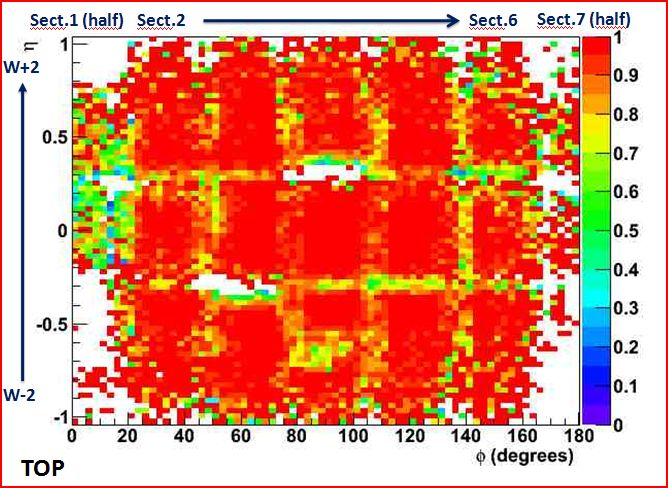
\includegraphics[width=0.9\textwidth]{eff_eta_phi_top_09_new}
       \caption{RPC trigger efficiency in CRAFT09 as a function 
       of $\eta$ and $\phi$ for tracks in the top part of the Barrel detector
      ($ 0^\circ < \phi < 180^\circ $). The $\eta$ and $\phi$
      coordinates are extrapolated to the reference layer.
      The wheels (sectors) corresponding to different $\eta$-$\phi$
      regions are labelled on the left (top) part of the plot.
}
    \label{fig:eff_eta_phi_top_09}
  \end{center}
\end{figure}


\begin{figure}[hbtp]
     \begin{center}
      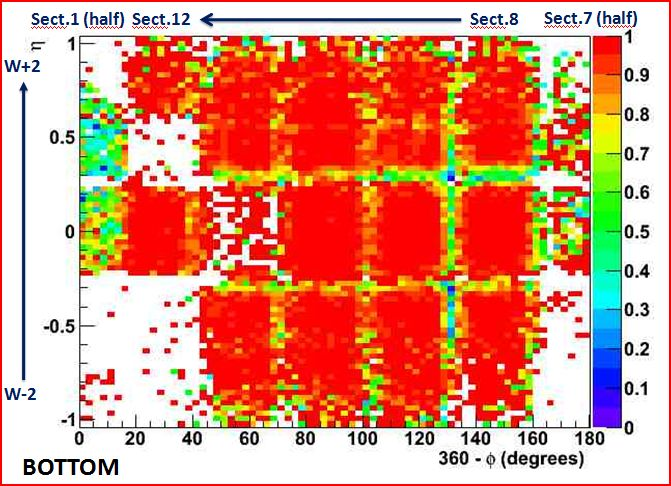
\includegraphics[width=0.9\textwidth]{eff_eta_phi_bot_09_new}
       \caption{RPC trigger efficiency iin CRAFT09 as a function of $\eta$ and $\phi$
       for tracks in the bottom part of the Barrel detector
       ($ 180^\circ < \phi < 360^\circ $). The $\eta$ and $\phi$ coordinates are
       extrapolated to the reference layer.
       Note that the variable plotted on the x-axis is
       $360^\circ - \phi$. The wheels (sectors) corresponding to different $\eta$-$\phi$
       regions are labelled on the left (top) part of the plot.
       }
    \label{fig:eff_eta_phi_bot_09}
  \end{center}
\end{figure}

In CRAFT09 runs all the RPCs are in readout and with higher
average efficiency, being many problems solved during
the CRAFT08 commissioning phase. This reflects in a general improvement of
performances. The less populated regions in the plot seem to be still
related to missing DT trigger matches in those regions.

Figure~\ref{fig:eff_pt_09_vs_08} shows the efficiency vs.
\pt for cosmics tracks in the fiducial region defined
by Table~\ref{tab:volumecuts}. 
The efficiency plateau is reached at around \pt $ > 20 \GeVc$ at 
a value $\epsilon_{09} = 98.01 \pm 0.08 % $.

\begin{figure}[hbtp]
  \begin{center}
    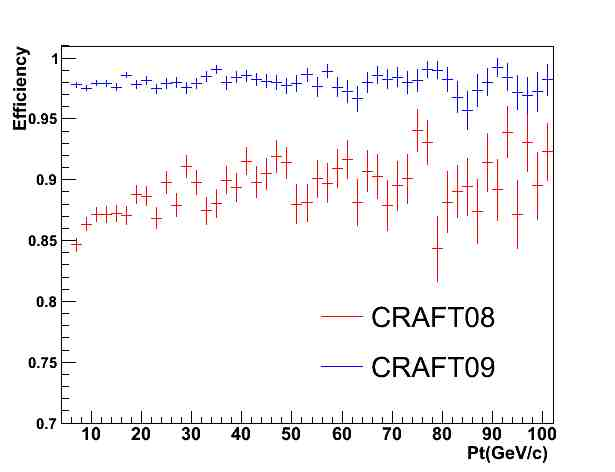
\includegraphics[width=0.8\textwidth]{eff_pt_09_vs_08}
    \hspace{1cm}
    \caption{Trigger efficiency vs. \pt of the tracks.
    The efficiency in CRAFT08 is also shown for comparison.
}
    \label{fig:eff_pt_09_vs_08}
  \end{center}
\end{figure}

\subsection{Comparison of CRAFT08 vs. CRAFT09 performances}
\label{comparison}
The results shown in the previous sections show a differece of about
$9 \% $ between the plateau efficiencies $\epsilon_{08}$ and $\epsilon_{09}$.
At the same time, as seen from Table~\ref{tab:runs}, also the average Barrel RPCs 
efficiency increases from $82.41\%$ in CRAFT08 to $92.05\%$ in CRAFT09, thanks
 to the HV increase from $9.2$ to $9.4$ kV and to the
 fixing of many problems during the commissioning 
effort in CRAFT08 (see also~\cite{ref:craft08pap}).

%The sensitivity of trigger performances 
%to the change of chambers efficiency from CRAFT08
%to CRAFT09 can be explained with the geometry of trigger
%towers, which has not been optimized for cosmic muons. For this reason,
%a fewer number of RPC is likely to be traversed by a cosmic track 
%2Bin a trigger cone with respect to a muon from collisions. For instance, if the average number 
%of chambers traversed by a track in a cone is 4, we get with a simple calculation 
%a trigger probability of $86.5\%$ for RPC 
%efficiency as of CRAFT08, and a trigger probability of 
%$97.3\%$ for RPC efficiency as of CRAFT09. 
To do a sistematic  study of the  dependancy of the trigger efficiency 
from the efficiency of the chambers the geometry of the  cones  
has to be taken into account.
%In any case, we do not expect such critical trigger behaviour in collisions because 
%of the highly optimized cones geometry and trigger patterns for these muons.

\section{Conclusions}
A method to measure the L1 RPC trigger efficiency has been developed.
It exploits as efficiency probes muon tracks matched to a DT trigger. 
It can be used to measure the trigger efficiency also for channels where 
there are not two back-to-back muons (W channels, top channel, etc.).
The method has been validated on CRAFT08 data by comparing with results 
based on the Tag and Probe technique, showing a good agreement.
The method has been applied to determine Barrel RPC trigger efficiencies 
on cosmics data in CRAFT08 and CRAFT09 samples, showing a significative 
improvement of the trigger efficiency in CRAFT09.
Further validation, to understand in particular the effect of possible 
residual correlations between DT and RPC triggers, can be done on Monte Carlo 
by comparing results with MC truth.
The algorythm has been included in the RPC Prompt Analysis framework.

%% References
\bibliography{auto_generated}

